\chapter{Discussion}
\paragraph{}
This chapter summarizes the experience of running usability testing of WebSlicer and the construction of a RepRap 3D printer that was used during software trials.

\section{Usability Testing}
\paragraph{}
Good design goes through many design iterations before it is considered production ready. 
Between iterations feedback is given through usability testing. 
For this research the time line was short thus, only one cycle of usability testing was completed.

\subsection{Task Description}
% paraphrase part E from IRB form
\paragraph{}
WebSlicer was evaluated by giving six research participants a series of tasks to preform in a controlled environment.
This environment consisted of a lab computer with a small collection of model files and a web browser.
The tasks that were given to participants are formalized in Table \ref{tab:tasks}.
Participants were also asked to fill out a questionnaire when they had completed the study.
This questionnaire asked participants to rate the level of difficulty of each task from 1 to 5 and to include comments of what they thought of each task.
Results of the average difficulty reported by users is shown in Table \ref{tab:tasks}.
As an incentive to participate, participants were given a small 3D printed figure of their choosing.

% table of user tasks
\begin{table}[h]
  \centering
    \begin{tabularx}{\textwidth}{ |l|l|l|X| }
      \hline
      Task \# & Task Name & Average Easiness & Description \\ \hline
      \hline
      1 & Create a new user & 4.66 out of 5 & Participants were simply asked to click a button which generated a unique ID for them. \\ \hline
      2 & Upload your file & 5 out of 5 & Uploading a model file of the participants choosing from a given USB drive. \\ \hline
      3 & Adjust slicer settings & 4.33 out of 5 & Participants were presented with a table of settings and their value. They were instructed to find these settings and change them while ignoring all other settings. \\ \hline
      4 & Analyze and download G-code & 4.66 out of 5 & This task simply required the user to toggle the visualizer to see the output of their actions in prior tasks. \\ \hline
    \end{tabularx}
  \caption{The tasks given to participants of the usability study. The participants were asked to complete the tasks in numerical order. Average easiness is the average of all participants responses where 5 was the easiest and 1 was the hardest.}
  \label{tab:tasks}
\end{table}

%\subsection{Testing Hypothesis}
\subsection{Results}
% what did i expect to see from this testing
\paragraph{}
The expected result of usability testing was to expose some minor flaws of the user interface (UI) design; however, the results showed that more than minor changes would be required before the next iteration of WebSlicer.
G-code output in textual form exposed to the user was found to be a bug in certain cases during usability testing.
The output when slicing certain models was so large that the browser crashed when trying to load the text to the screen.
This bug could be resolved by filtering the amount of text displayed at one time to the user.

\paragraph{}
Another flaw that was exposed during testing was the functionality of the G-code visualizer.
Most participants found that both the controls, and explanation of what it was meant to accomplish was lacking as shown in Figure \ref{fig:visualizer}.
One proposed solution would be to replace the numerical input fields with sliders which gives more natural control.
Concluded from this is that more textual explanations and user guidance was required in further iterations of WebSlicer.

\begin{figure}[!ht]
  \centering
  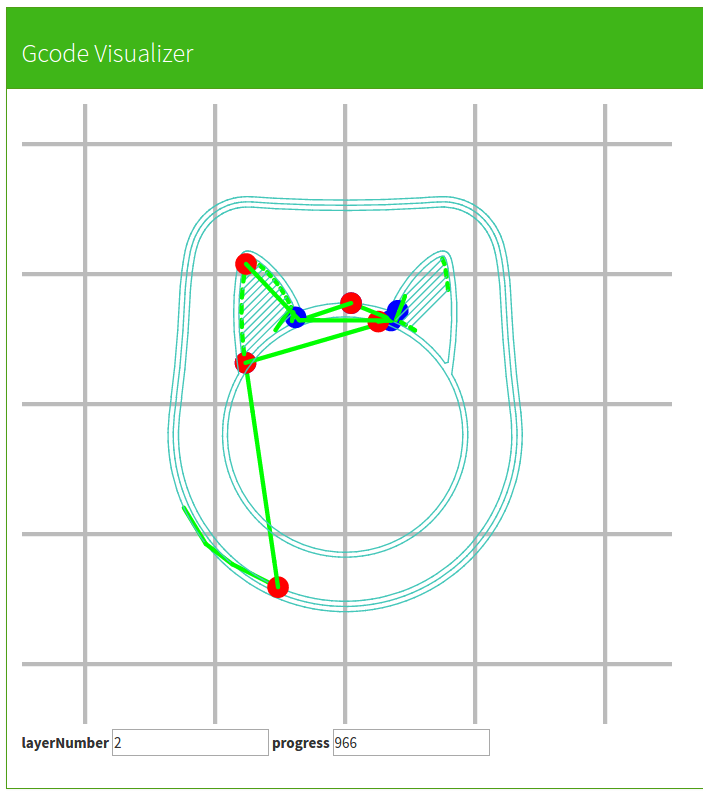
\includegraphics[width=\linewidth]{images/visualizer.png}
  \caption{This is what the output from the visualizer looks like to the user after successfully slicing a model.}
  \label{fig:visualizer}
\end{figure}

\begin{figure}[!ht]
  \centering
  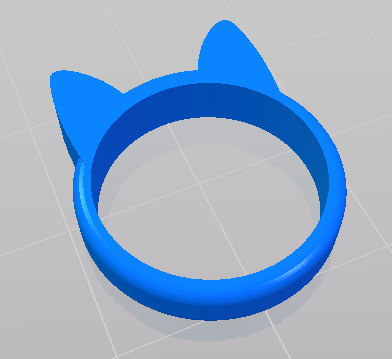
\includegraphics[width=\linewidth]{images/cat-ring.png}
  \caption{This is the 3D model that Figure \ref{fig:visualizer} is representing in G-code.}
  \label{fig:cat-ring}
\end{figure}

\section{Printer Build}
\paragraph{}
For this research a 3D printer was required to test the output of the slicer.
Instead of purchasing an expensive pre-built machine, a RepRap style 3D printer was constructed using commonly available materials as shown in Figures \ref{fig:print1} and \ref{fig:print2}.
Building the printer took approximately 3 months and incurred many issues along the way such as faulty electronics and bad wiring.
During the research when testing parameters were required for the slicer those from this printer were used.
Additionally, all the incentive parts that were given to research participants for their service during usability testing were printed on this machine.

\paragraph{}
The design of the 3D printer is that of a Cartesian RepRap Prusia i3 variant.
The frame is built of extruded aluminum bar and all complex mechanical parts were 3D printed on another machine.
The electronics consisted of an old computer power supply, Raspberry Pi, Arduino Mega, and a salvaged PID controller in addition to a standard set of heaters and motors.
Octoprint was installed on the Raspberry Pi and was used during the Octoprint integration with the client side of WebSlicer.

\begin{figure}[t]
  \centering
  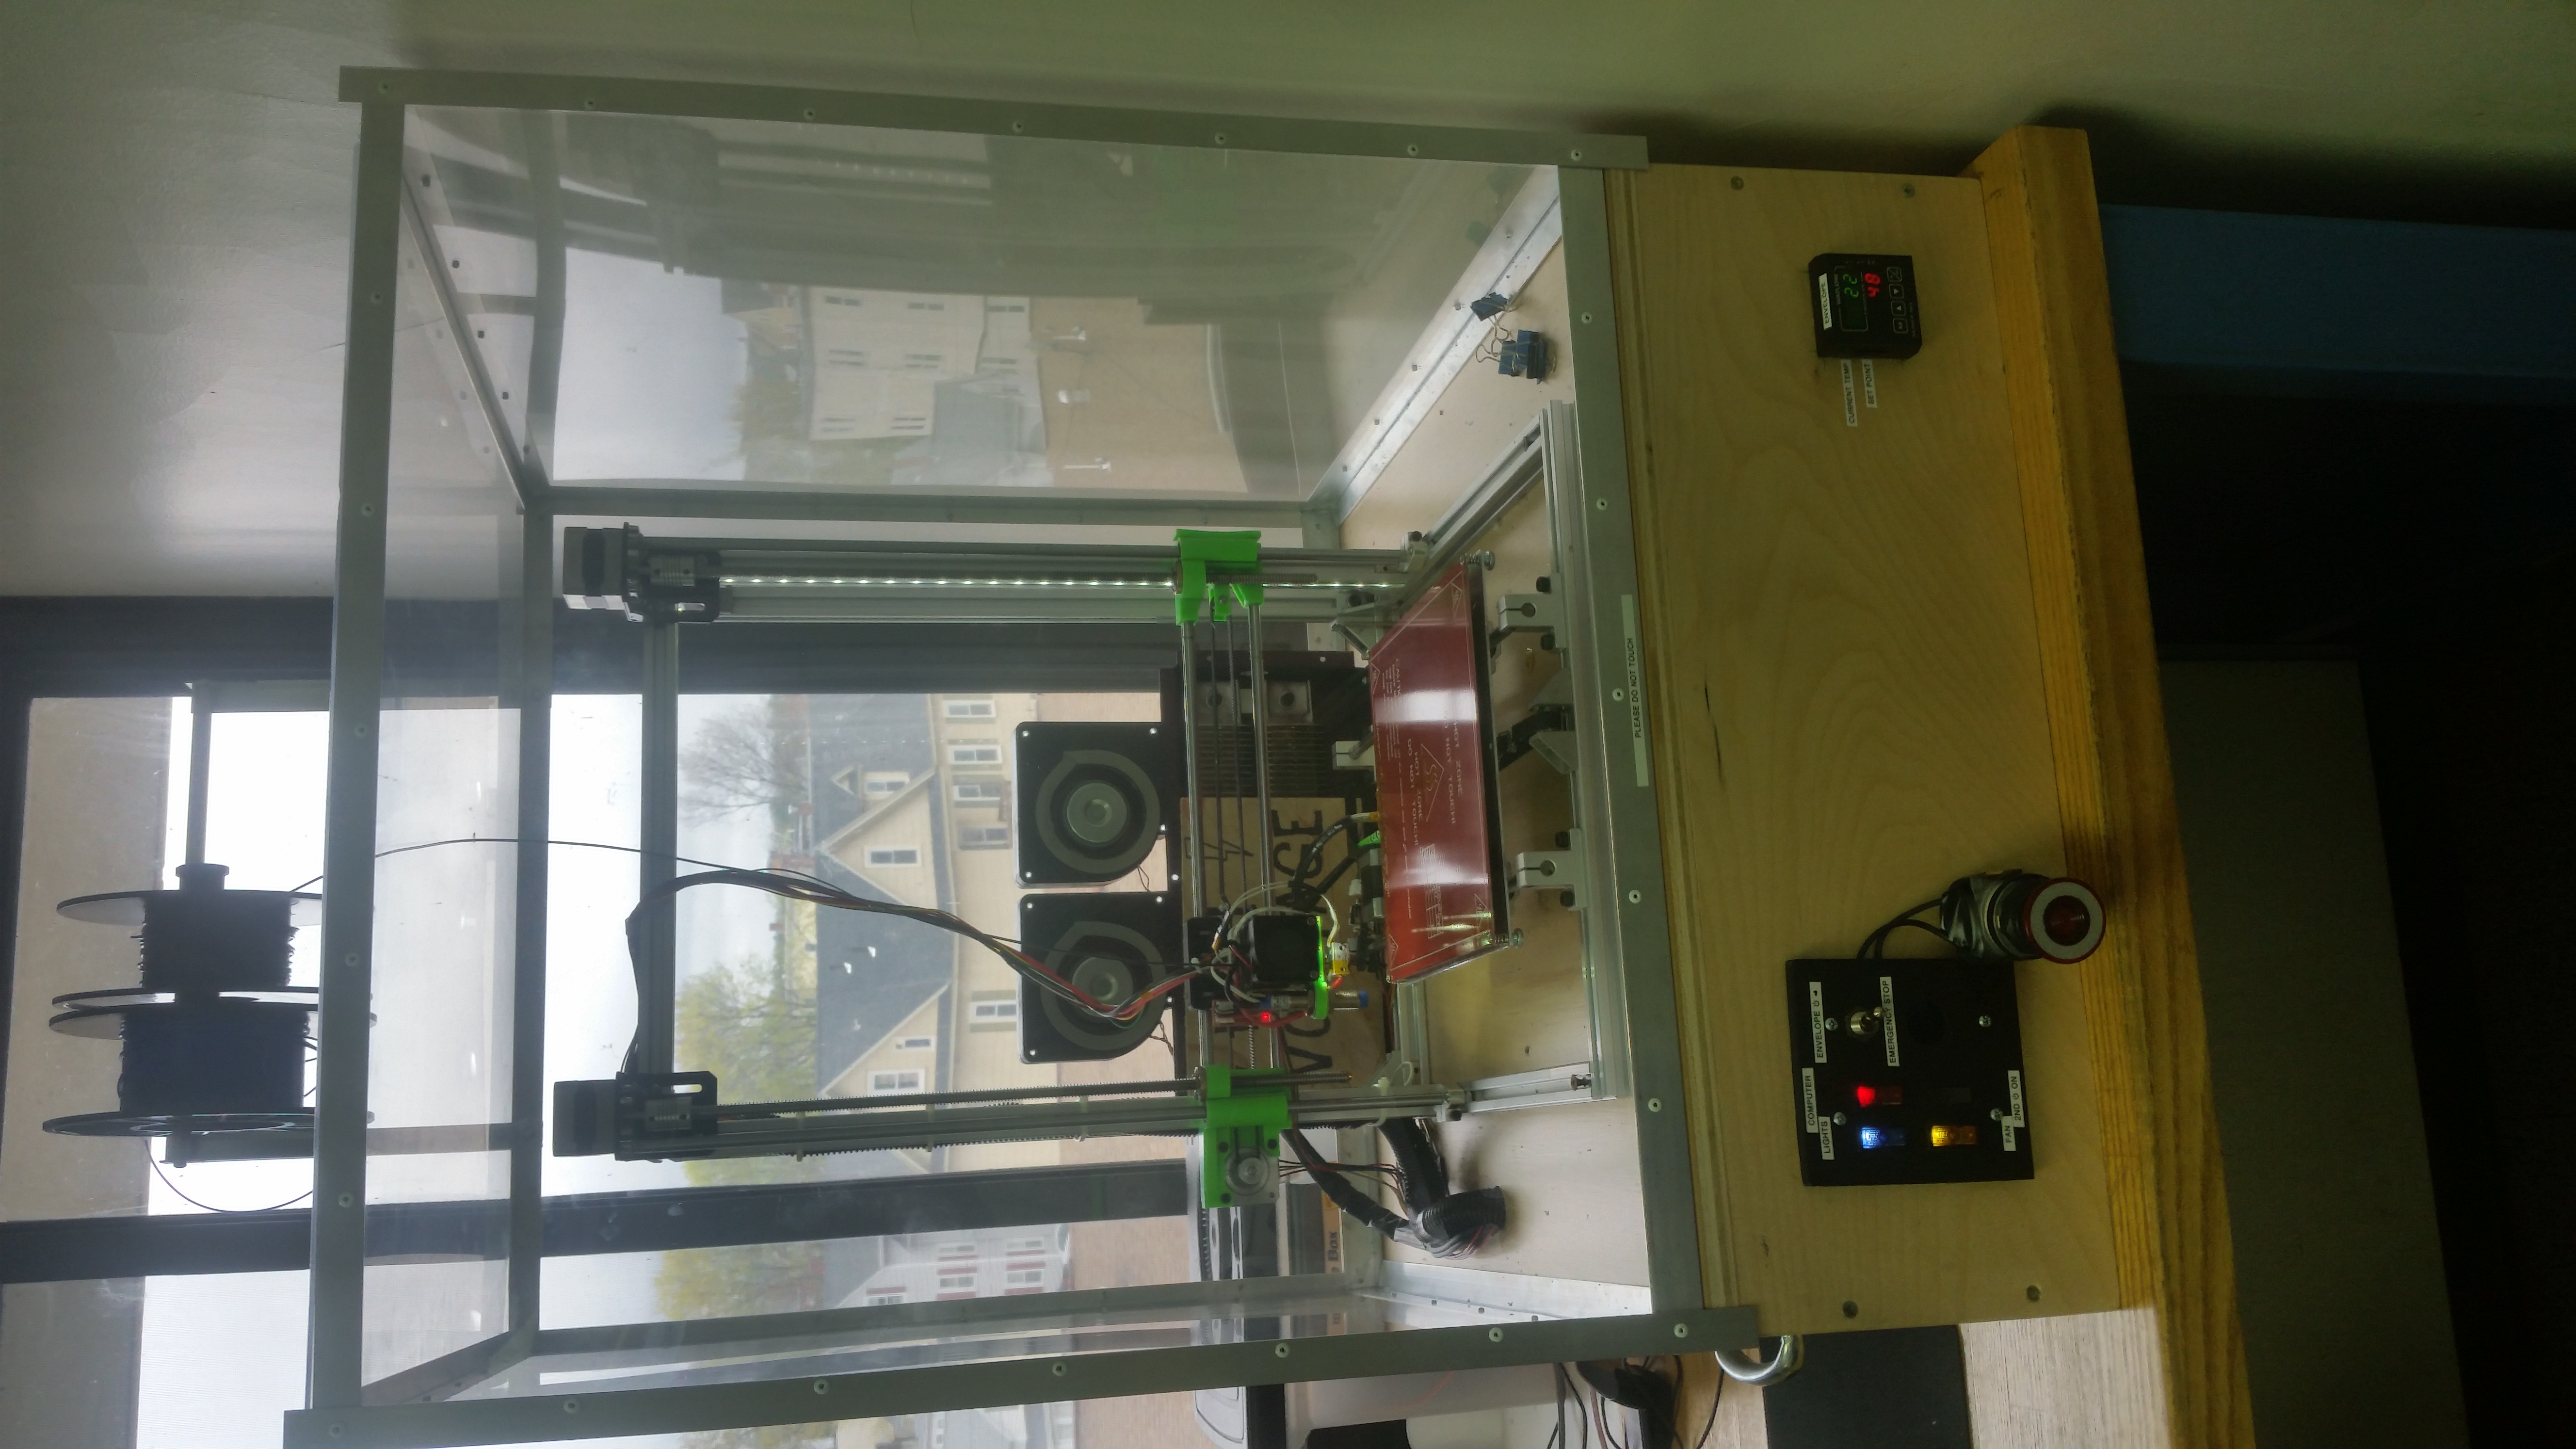
\includegraphics[width=\linewidth, angle=-90]{images/print1.jpg}
  \caption{RepRap style 3D printer that was built for this research (front view)}
  \label{fig:print1}
\end{figure}

\begin{figure}[t]
  \centering
  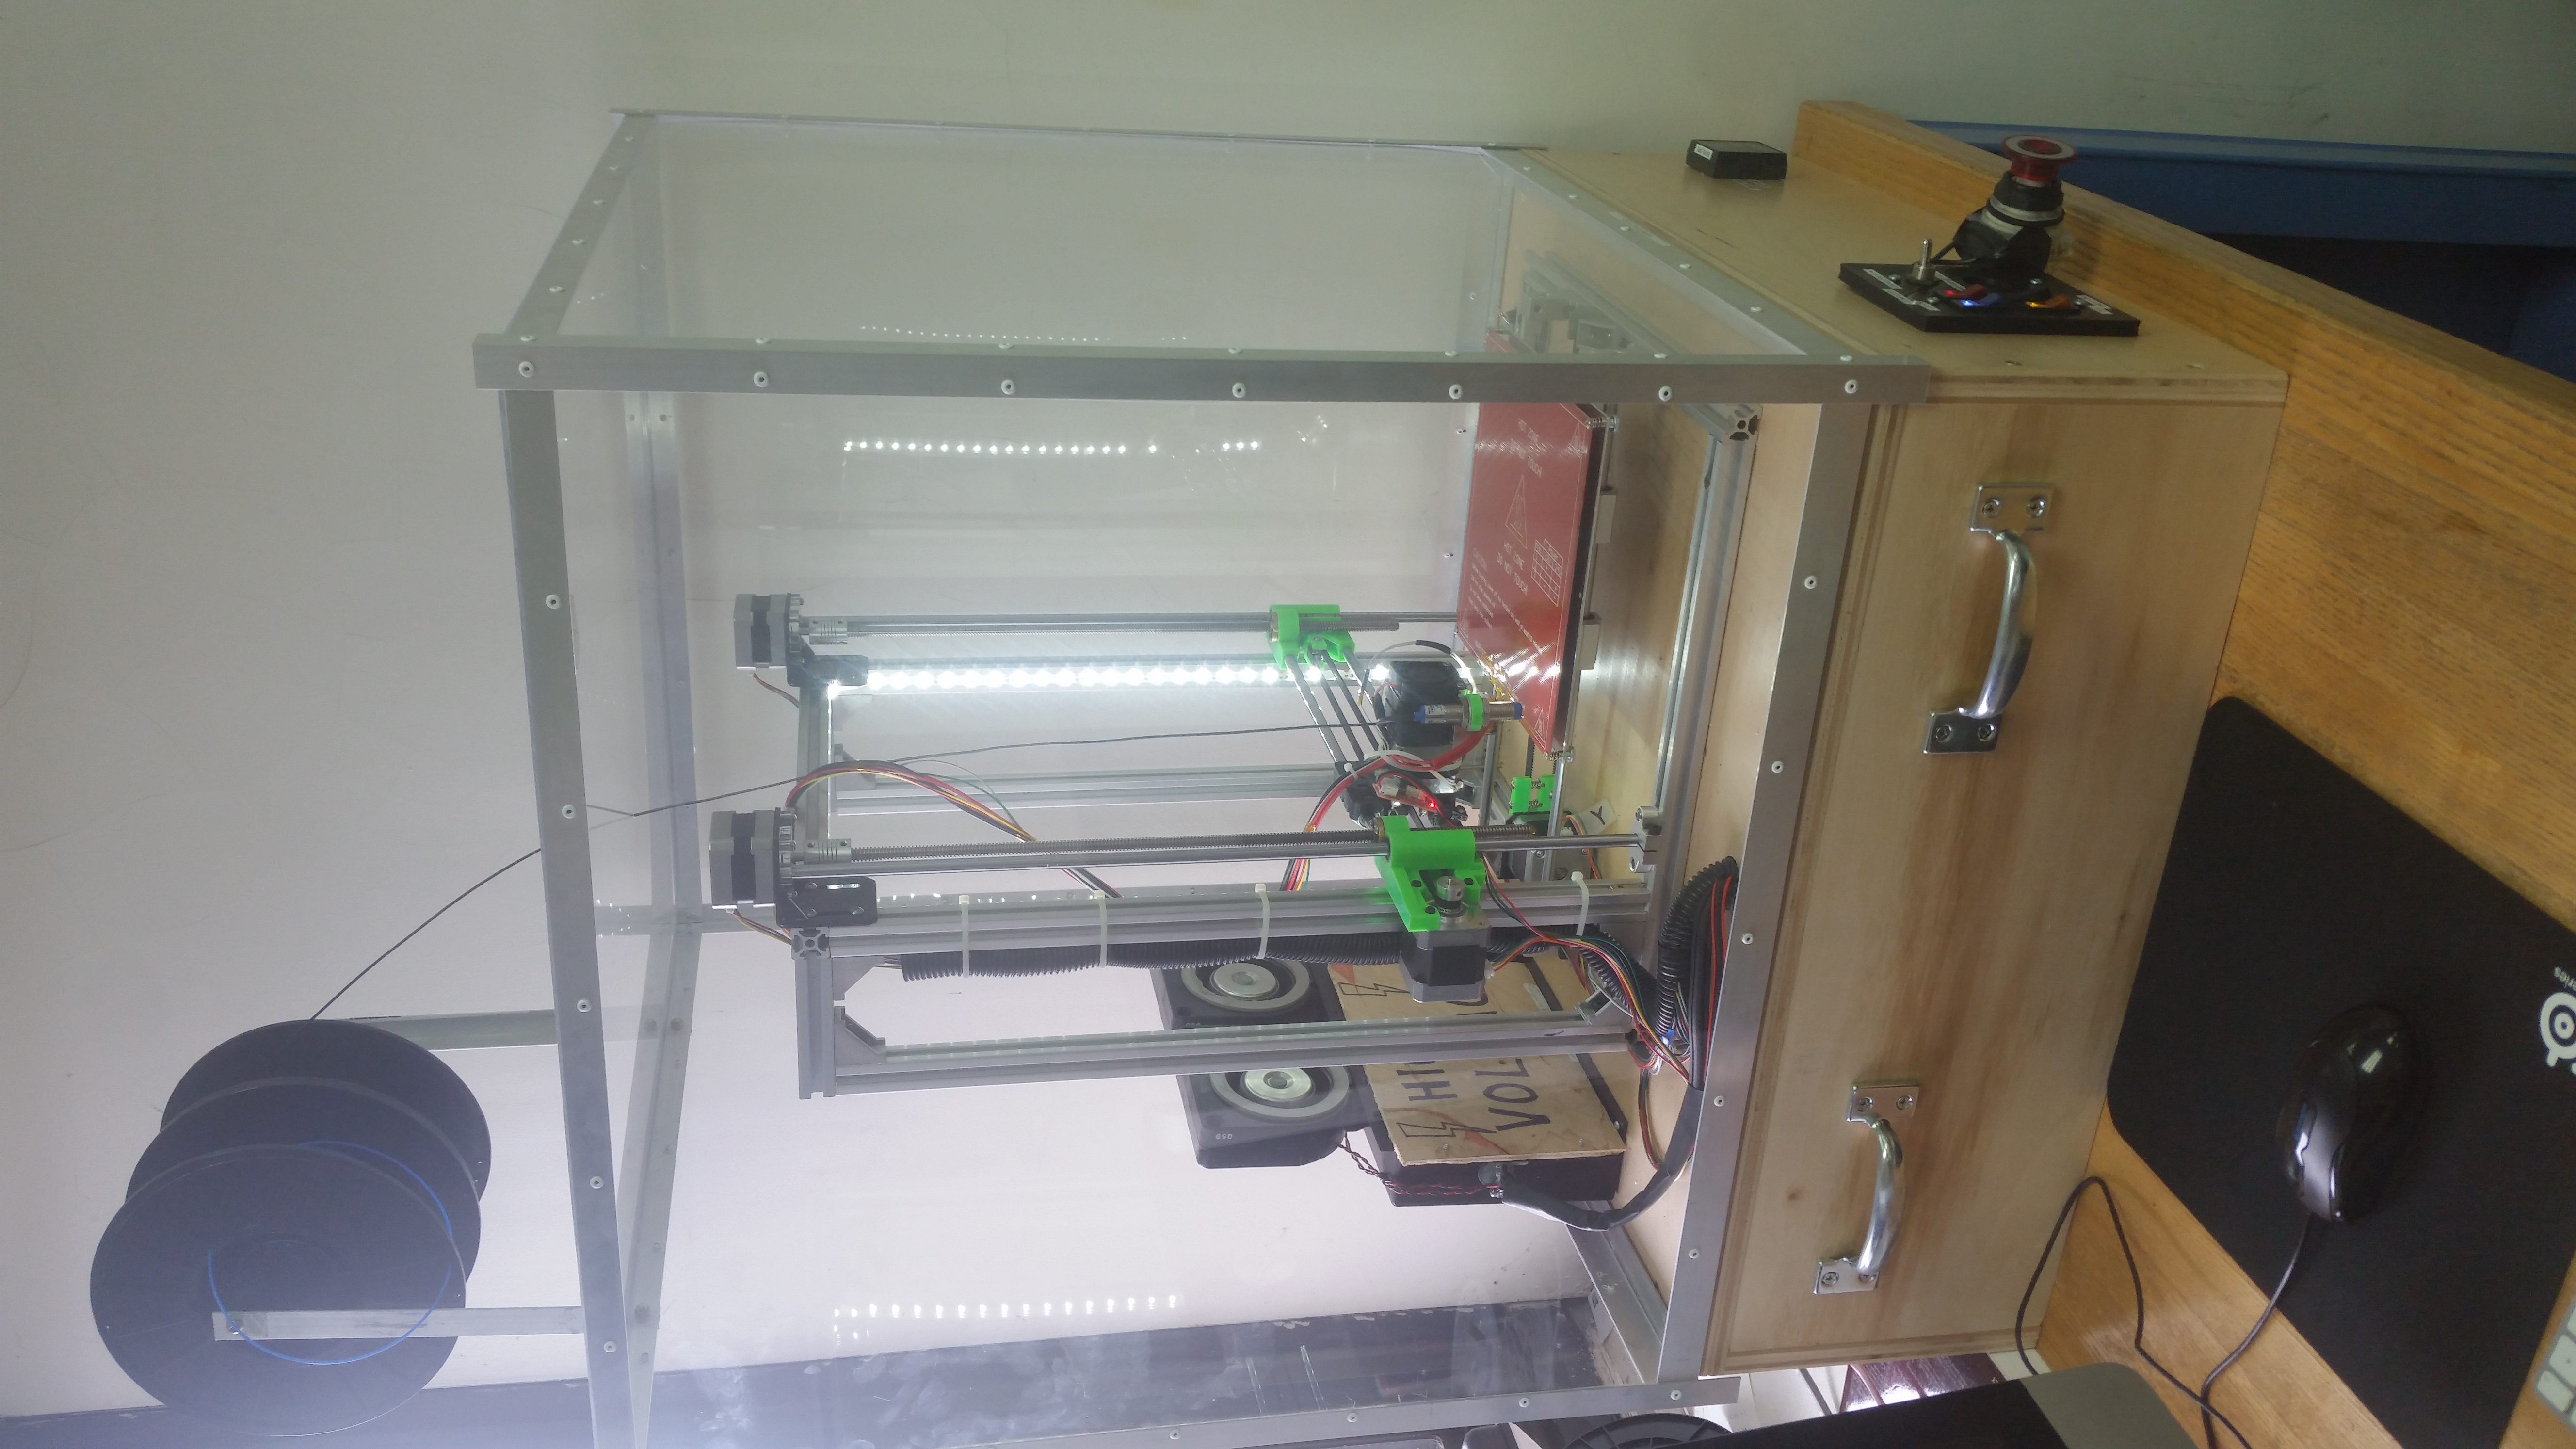
\includegraphics[width=\linewidth, angle=-90]{images/print2.jpg}
  \caption{RepRap style 3D printer that was built for this research (side view)}
  \label{fig:print2}
\end{figure}

\section{Future of WebSlicer}
\paragraph{}
The goal of future versions of WebSlicer are to lay the groundwork for a larger manufacturing software tool.
This manufacturing software will link together many 3D printers and allow for unified control from a web based hub.
Unified control such as this would allow for users to preform small scale manufacturing which would fill a void that currently exists in the manufacture of plastic parts.